\documentclass{standalone}
\usepackage{tikz}
\usetikzlibrary{
  arrows,
  automata,
  fit,
  positioning
}
\tikzset{
  ->,
  >=stealth,
  node distance = 0.5cm and 1cm,
  every state/.style = {thick},
  initial text = $ $,
}

\begin{document}
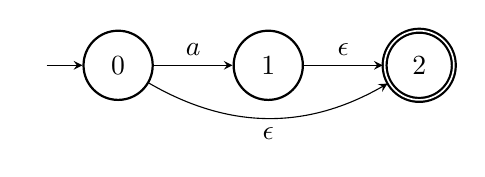
\begin{tikzpicture}[baseline=0]
  \node[state, initial] (0) {$0$};
  \node[state, right=of 0] (1) {$1$};
  \node[state, right=of 1, accepting] (2) {$2$};
  \draw
      (0) edge[above] node{$a$} (1)
      (0) edge[below, bend right] node{$\epsilon$} (2)
      (1) edge[above] node{$\epsilon$} (2);
\end{tikzpicture}
\end{document}
